\chapter{Nanosheared electrolyte}

\vspace{-1cm} \noindent \textcolor{graytitle}{\textit{{\Large Aqueous NaCl solution sheared by two walls}}\vspace{0.5cm} }

\noindent \hspace{-0.45cm}\begin{wrapfigure}{r}{4cm}
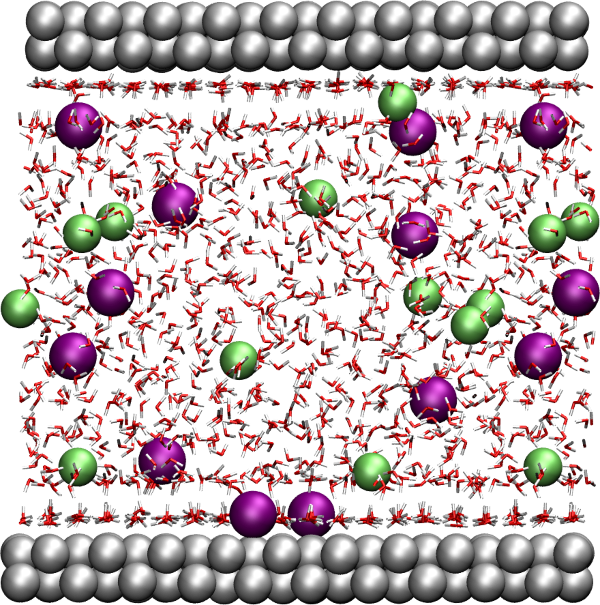
\includegraphics[width=4cm]{tutorials/level2/nanosheared-electrolyte/nanoconfined-electrolyte-light.png}
\end{wrapfigure}

\noindent The objective of this tutorial is to
simulate an electrolyte sheared by two walls. Some properties
of the sheared fluid, such as the time-averaged velocity profile
will be extracted. 
This tutorial illustrates the important aspects of
combining a fluid and a solid in the same simulation.

\section{System generation}

\noindent Create a new folder called \textit{SystemCreation/}. Within \textit{SystemCreation/},
open a blank file called \textit{input.lammps}, and copy 
the following lines into it:

\begin{lcverbatim}
# LAMMPS input file
units real
atom_style full
bond_style harmonic
angle_style harmonic
pair_style lj/cut/tip4p/long 1 2 1 1 0.1546 12.0
kspace_style pppm/tip4p 1.0e-4
\end{lcverbatim}

\noindent These lines are used to define the most basic parameters,
including the \textit{atom}, \textit{bond}, and \textit{angle} styles, as well as 
interaction potential (here Lennard Jones with cut-off and long 
range Coulombic) and long range solver (here PPPM). 
These lines are relatively similar to the 
previous tutorial (:ref:`all-atoms-label`).

\begin{tcolorbox}[colback=mylightblue!5!white,colframe=mylightblue!75!black,title=About lj/cut/tip4p/long pair style]
The lj/cut/tip4p/long pair style is similar to the conventional 
Lennard Jones + Coulomb interaction, except that it is made specifically 
for four point water model (tip4p). The atom of the water model
will be type 1 (O) and 2 (H). All the other atoms of the simulations 
are treated \textit{normally} with long range coulomb interaction.
\end{tcolorbox}

\noindent Let us create the box:

\begin{lcverbatim}
# ------------- System definition
lattice fcc 4.04
region box block -4 4 -4 4 -13 13
create_box 5 box &
\end{lcverbatim}

\noindent The \textit{lattice} command defines the unit
cell. Here, the face-centered cubic (fcc) lattice with a scale factor of
4.04 has been chosen for the future positioning of the atoms
of the walls.

The \textit{region} command defines a geometric
region of space. By choosing \textit{xlo=-4} and \textit{xhi=4}, and
because we have previously chosen a lattice with scale
factor of 4.04, the region box extends from -16.16 Å to 16.16 Å.

The \textit{create$\_$box} command creates a simulation box with 5 types of atoms in
the simulation. This command extends over 6 lines thanks to the
$\&$ character. The second and third lines are used to
specify that the simulation contains 1 type of bond and 1
type of angle (both required by the water molecule). The parameters of
these bond and angle constraints will be given later. The
three last lines are for memory allocation.
Note that 5 atom types are needed for respectively the oxygen and hydrogen
of the water molecules, the two types of ions ($\text{Na}^+$, $\text{Cl}^-$), and the
single atom type of the walls.

Now, we can add atoms to the system. First, let us create two
sub-regions corresponding respectively to the two solid
walls, and create a larger region from the union of the two
regions. Then, let us create atoms of type 5 (the wall) within the two
regions:

\begin{lcverbatim}
# create the walls
region rbotwall block -4 4 -4 4 -12 -10
region rtopwall block -4 4 -4 4 10 12
region rwall union 2 rbotwall rtopwall
create_atoms 5 region rwall
\end{lcverbatim}

\noindent Atoms will be placed at the positions of the previously
defined lattice.
In order to add the water molecules, we first need to
download the \href{../../../../../inputs/level2/nanosheared-electrolyte/TIP4P2005.txt}{TIP4P2005.txt}
file and place it in \textit{SystemCreation/}. It contains all the
necessary information about the water molecule, such as
atom positions, bonds, and the angle.

Add the following lines
to input.lammps:

\begin{lcverbatim}
# create the fluid
region rliquid block -4 4 -4 4 -9 9
molecule h2omol ../TIP4P2005.txt
lattice sc 4.04
create_atoms 0 region rliquid mol h2omol 482793
\end{lcverbatim}

\noindent Withing the last four lines, a \textit{region} named \textit{rliquid} for depositing the water molecules is created based
on the last defined lattice, which is \textit{fcc 4.04}. 
The \textit{molecule} command opens up the \textit{TIP4P2005.txt} file, and names
the associated molecule \textit{h2omol}.
A new simple cubic lattice is defined in order to place the water
molecules on it, with a distance of 4.04 Ångstroms between
each water molecule. Note that the new lattice replaces the
previous one, as LAMMPS reads a script from top to bottom.
Note that the distance of 4.04 Ångstroms is larger than the typical
equilibrium distance between water molecules in a liquid,
but this will allow us to insert ions more safely (see below). 
Finally, molecules are created on the sc lattice by the \textit{create$\_$atoms} command. The
first parameter is '0' because we use the atom id from the
\textit{TIP4P2005.txt} file. The number \textit{482793} is a seed that is
required by LAMMPS, it can be any positive integer.
Let us create 20 ions (10 $\text{Na}^+$ and 10 $\text{Cl}^-$)
in between the water molecules:

\begin{lcverbatim}
# create the ions
create_atoms 3 random 10 52802 rliquid overlap 0.3 maxtry 500
create_atoms 4 random 10 90182 rliquid overlap 0.3 maxtry 500
set type 3 charge 1.0
set type 4 charge -1.0
\end{lcverbatim}

\noindent Each \textit{create$\_$atoms} command will add 10 ions at random positions
within the 'rliquid' region. Feel free to increase or decrease the salt
concentration by changing the number of desired ions.
The charges of the newly added ions are specified by the two \textit{set} commands.
To keep the system charge neutral, always insert the same number of 
$\text{Na}^+$ and $\text{Cl}^-$ (unless of course there are other charges in the system).
We need to define the parameters of the simulation: the mass
of the 6 atoms (O, H, $\text{Na}^+$, $\text{Cl}^-$, and wall), the
pairwise interaction parameters (here the parameters for the
Lennard-Jones potential), and the bond and angle parameters.
Copy the following line into input.lammps:

\begin{lcverbatim}
# settings
include ../PARM.lammps
\end{lcverbatim}

\noindent Create a new text file, call it \textit{PARM.lammps}, and copy it
next to the \textit{SystemCreation/} folder. Copy the following lines
into PARM.lammps:

\begin{lcverbatim}
# Parameter file
mass 1 15.9994 # water
mass 2 1.008 # water
mass 3 28.990 # ion
mass 4 35.453 # ion
mass 5 26.9815 # wall
pair_coeff 1 1 0.185199 3.1589 # water
pair_coeff 2 2 0.0 0.0 # water
pair_coeff 3 3 0.04690 2.4299 # ion
pair_coeff 4 4 0.1500 4.04470 # ion
pair_coeff 5 5 11.697 2.574 # wall
bond_coeff 1 0 0.9572 # water
angle_coeff 1 0 104.52 # water

\end{lcverbatim}

\noindent Each \textit{mass} command assigns a mass in grams/mole to an atom type. Each
\textit{pair$\_$coeff} assigns respectively the depth of the potential
(in Kcal/mole), and the distance (in Ångstrom) at which the
particle-particle potential energy is 0.

\begin{tcolorbox}[colback=mylightblue!5!white,colframe=mylightblue!75!black,title=About the parameters]
The parameters for water
correspond to the TIP4P/2005 water model, and the parameters
for $\text{Na}^+$ and $\text{Cl}^-$  are
taken from the CHARMM-27 force field.
\end{tcolorbox}

\noindent Only pairwise interaction between atoms of
identical type were assigned. By default, LAMMPS calculates
the pair coefficients for the interactions between atoms
of different types (i and j) by using geometrical
average: $\epsilon_{ij} = \epsilon_i + \epsilon_j)/2$, 
$\sigma_{ij} = (\sigma_i + \sigma_j)/2.$
Other rules for cross coefficients can be set with the
\textit{pair$\_$modify} command, but for the sake of simplicity,
let us keep the default option here.
The bond coefficient (here for the O-H bond of the water
molecule) sets respectively the energy of the harmonic
potential and the equilibrium distance in Ångstrom. The
value is '0' for the energy, because we are going to use a
rigid model for the water molecule. The shape of the
molecule will be preserved later by the shake algorithm.
Similarly, the angle coefficient (here for the H-O-H angle
of the water molecule) sets the energy of the harmonic
potential (also 0) and the equilibrium angle is in degree.
Finally, add the following lines to the input file:

\begin{lcverbatim}
# run
run 0
write_data system.data
write_dump all atom dump.lammpstrj
\end{lcverbatim}

\noindent With \textit{run 0}, the simulation will run for 0 step,
enough for creating the system and saving the final state.
The \textit{write$\_$data} finally creates a file named \textit{system.data}
containing all the information required to restart the
simulation from the final configuration generated by this
input file.
The \textit{write$\_$dump} command print the final
positions of the atoms, and can be used with VMD or ovito
to visualize the system.
This input script is ready to be ran with LAMMPS. When the
run is over, open the log file and make sure that atoms have
been created (look for lines like 'Created 3648 atoms'), or
just look at the dump file with VMD:

\begin{figure}
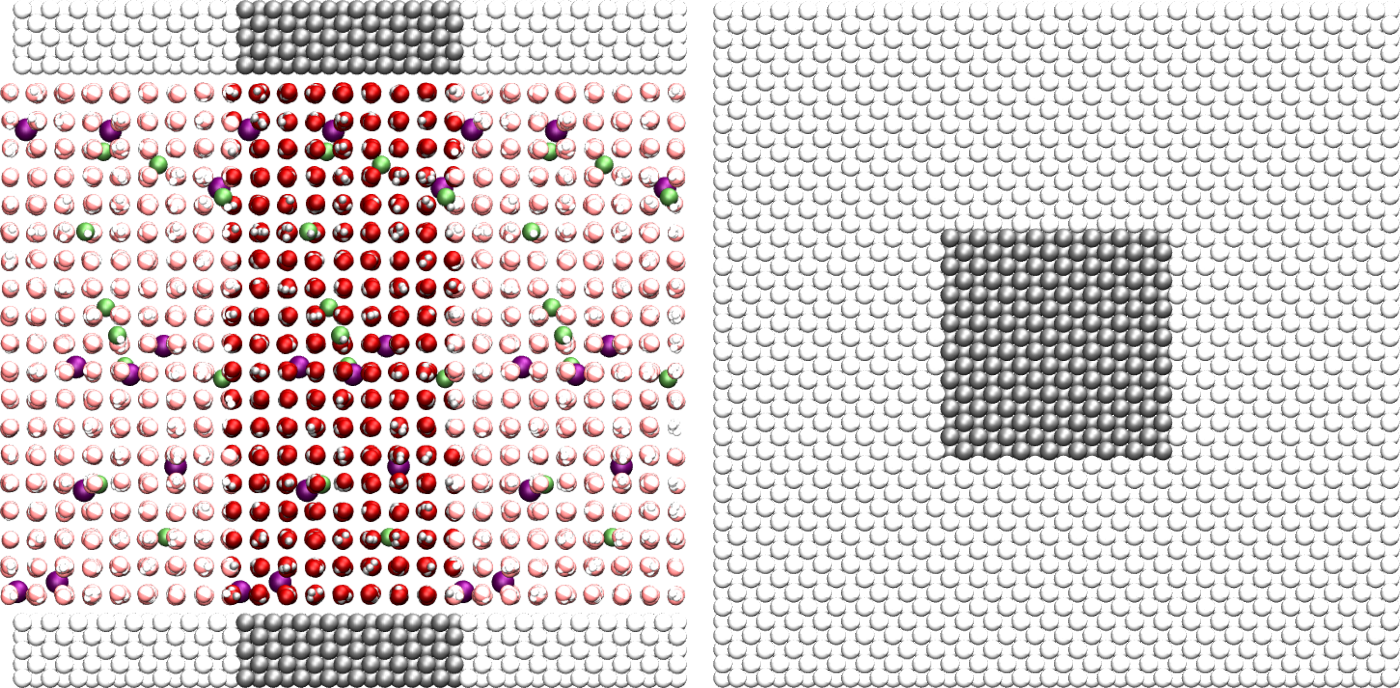
\includegraphics[width=\linewidth]{tutorials/level2/nanosheared-electrolyte/systemcreation-light.png}
\end{figure}

Always check that your system has been correctly created
by showing the periodic images. Atomic defects often
occur at the boundary.

\section{Energy minimization}

\noindent \begin{tcolorbox}[colback=mylightblue!5!white,colframe=mylightblue!75!black,title=Why is energy minimization necessary?]
It is clear from the way the system has been created that
the atoms are not at equilibrium distances from each
others. Indeed, some of the ions added using the \textit{create$\_$atoms}
commands are too close to the water molecules.
If we were to start a molecular dynamics
simulation now (i.e. solve the equations of motion) with
a conventional timestep of 1 femto-seconds, the atoms
would exert huge forces on each others, accelerate
brutally, and the simulation would fail.
\end{tcolorbox}

\noindent \begin{tcolorbox}[colback=mylightblue!5!white,colframe=mylightblue!75!black,title=Dealing with overlapping atoms]
MD simulations failing due to overlapping atoms are
extremely common, and I can almost guarantee that you
will face a similar issue at some point. If it occurs,
you can either
\begin{itemize}
\item delete the overlapping atoms using the \textit{delete$\_$atoms} command of LAMMPS, or
\item move the atoms to more reasonable distances before the simulation starts.
\end{itemize}
\end{tcolorbox}

\noindent Let us move the atoms and place them
in more energetically favorable positions before starting the simulation.
To perform the energy minimization with our system, let us
create a new folder named Minimization/, and create a new
input file named input.lammps in it. The first lines will be
very similar to the previous input file:

\begin{lcverbatim}
# Initialisation
boundary p p p
units real
atom_style full
bond_style harmonic
angle_style harmonic
pair_style lj/cut/tip4p/long 1 2 1 1 0.1546 12.0
kspace_style pppm/tip4p 1.0e-4
# System definition
read_data ../SystemCreation/system.data
# settings
include ../PARM.lammps
\end{lcverbatim}

\noindent The only difference with the previous input is that, instead
of creating a new box and new atoms, we open the
previously created file \textit{system.data} located in \textit{SystemCreation/}.
\textit{system.data} contains the definition of the simulation box and the positions of the atoms.
Next, let us create a group for the water:

\begin{lcverbatim}
group gH2O type 1 2
\end{lcverbatim}

\noindent Creating groups will allow us to apply different dynamics and constraints to the
liquid and to the walls.
Let us also print the atoms positions in a dump file:

\begin{lcverbatim}
dump mydmp all atom 1000 dump.lammpstrj
\end{lcverbatim}

\noindent Now, we can include the most important commands for the
minimization:

\begin{lcverbatim}
fix mynve all nve/limit 0.1
fix myber all temp/berendsen 1 1 1
\end{lcverbatim}

\noindent The fix \textit{nve/limit} performs constant NVE integration to
update positions and velocities of the atoms at each
timestep, but limit the maximum motion an atom can do at
every timestep. The temp/berendsen fix rescales the
velocities of the atoms every timestep in order to reset the
temperature.

Since we want to perform a minimization step, both initial
and final temperatures have been chosen equal to 1K. The
third parameter is the damping factor, in time units, which
determines how rapidly the temperature is relaxed. Such
damping factor of 1 fs would be too small for a regular
molecular dynamics simulation, but is acceptable for a
minimization step during which we just want the atoms to
move slightly from their initial positions.

If we were to run the simulation as it is, it would fail
because nothing maintains the shape of the water molecules
(and the bond and angle energies are equal to 0). Let us use
the shake algorithm in order to maintain the shape of the
molecules. In addition, let us add a fix \textit{recenter} in order
to maintain the system centered in the middle of the box in
the \textit{z} direction:

\begin{lcverbatim}
fix myshk gH2O shake 1.0e-4 200 0 b 1 a 1
fix myrct all recenter NULL NULL INIT
\end{lcverbatim}

\noindent Fix recenter has no influence on the dynamics, but will keep the system in the 
center of the box, which makes the visualization easier.
Finally, let us choose a small timestep (because we
anticipate that the atoms are initially too close to each
others) and run for 10000 steps:

\begin{lcverbatim}
timestep 0.5
thermo 50
run 10000
write_data system.data
\end{lcverbatim}

\noindent When running the input.lammps file, you should see that the
total energy of the system decreases as expected (fifth
colum):

\begin{lcverbatim}
Step   Temp          E_pair         E_mol          TotEng         Press     
50   3.492673      -107825.17      0             -107786.32     -19733.701    
100   2.6260191     -108926.18      0             -108896.97     -20225.668    
150   2.2025292     -109692.83      0             -109668.34     -20319.962 
(...)
9800   1.0233163     -120975.23      0             -120963.85     -12590.345    
9850   1.022532      -120988.11      0             -120976.74     -12582.803    
9900   1.0222164     -121000.48      0             -120989.11     -12573.028    
9950   1.0215887     -121012.78      0             -121001.42     -12562.843    
10000   1.0206449     -121024.53      0             -121013.18     -12551.132 
\end{lcverbatim}

\noindent You can easily import log file into \textit{Python} using the
\href{https://pypi.org/project/lammps-logfile/}{LAMMPS logfile} tool, and plot the thermodynamic quantities as a function 
of the time:

\begin{figure}
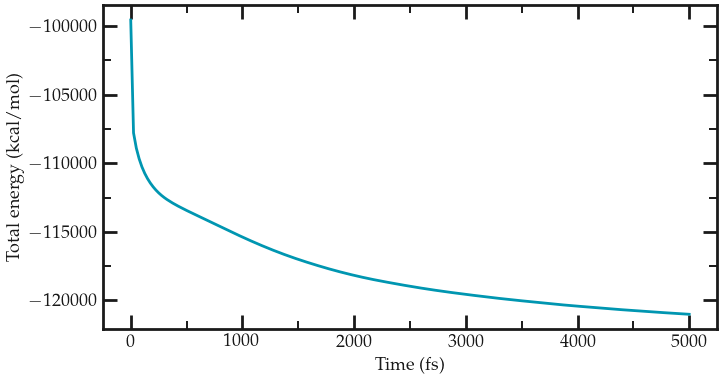
\includegraphics[width=\linewidth]{tutorials/level2/nanosheared-electrolyte/minimization-light.png}
\end{figure}

If you look at the trajectory using VMD, you will see some
of the atoms (the one that where initially in a problematic
position) slightly move from each others, as seen in \href{https://youtu.be/JWGZnFN4TOo}{this video}.

\section{System equilibration}

\noindent Now, let us properly equilibrate the system by letting both
fluid and piston relax at ambient temperature.
Create a new folder called \textit{Equilibration/}, create a new
input file in it, and add the following lines:

\begin{lcverbatim}
# Initialisation
boundary p p p
units real
atom_style full
bond_style harmonic
angle_style harmonic
pair_style lj/cut/tip4p/long 1 2 1 1 0.1546 12.0
kspace_style pppm/tip4p 1.0e-4
# System definition
read_data ../Minimization/system.data
# Simulation settings
include ../PARM.lammps
# Define groups
group gH2O type 1 2
group gNa type 3
group gCl type 4
group gliquid type 1 2 3 4
group gwall type 5
region rtop block INF INF INF INF 0 INF
region rbot block INF INF INF INF INF 0
group gtop region rtop
group gbot region rbot
group gwalltop intersect gwall gtop
group gwallbot intersect gwall gbot
\end{lcverbatim}

\noindent Here, several groups have been defined in order to differentiate
between solid, liquid (salt+water), $\text{Na}^+$, etc. (although
not all of them are used). In addition, groups containing only the
top wall (gwalltop) and the bottom wall (gwallbot) have been
created using the intersect keyword: the intersection
between all the atom on the top part of the box (gtop) and
all the atom of type 5 (gwall) corresponds to the top wall.
Then, add the following lines for the visualisation :

\begin{lcverbatim}
# visualisation
dump mydmp all atom 1000 dump.lammpstrj
thermo 50
variable walltopz equal xcm(gwalltop,z)
variable wallbotz equal xcm(gwallbot,z)
variable deltaz equal v_walltopz-v_wallbotz
fix myat1 all ave/time 10 10 100 v_deltaz file interwall_distance.dat
\end{lcverbatim}

\noindent The two variables allow to extract the centers of mass of
the two walls, respectively, and the deltaz variable
calculates the difference between the two centers of mass.
Finally, add the end of the input:

\begin{lcverbatim}
# Dynamics
fix mynve all nve
compute tliq gliquid temp
fix myber1 gliquid temp/berendsen 300 300 100
fix_modify myber1 temp tliq
compute twall gwall temp
fix myber2 gwall temp/berendsen 300 300 100
fix_modify myber2 temp twall
fix myshk gH2O shake 1.0e-4 200 0 b 1 a 1
fix myrct all recenter NULL NULL INIT
timestep 1.0
run 20000
write_data system.data
\end{lcverbatim}

\noindent The main differences with the previous step (minimize) are
the timestep of 1 fs instead of 0.5 fs, the thermostat that imposes a temperature of 300 K, for which the
fluid is expected to behave as a liquid, and the two thermostats are used instead of one:
one for the fluid, one for the solid (the use of \textit{fix$\_$modify} ensures
that the right temperature is used by the temp/berenden).

Run the input script. Note, I am running on 4 CPU cores using:

\begin{lcverbatim}
mpirun -np 4 lmp -in input.lammps
\end{lcverbatim}

\noindent To complete the 20000 steps (20 ps), it takes about 6 minutes. The duration 
may differ on your computer.
The distance between the two walls
reduces until it reaches an equilibrium value, see the evolution
of the distance between the walls (printed in a data file by fix myat1):

\begin{figure}
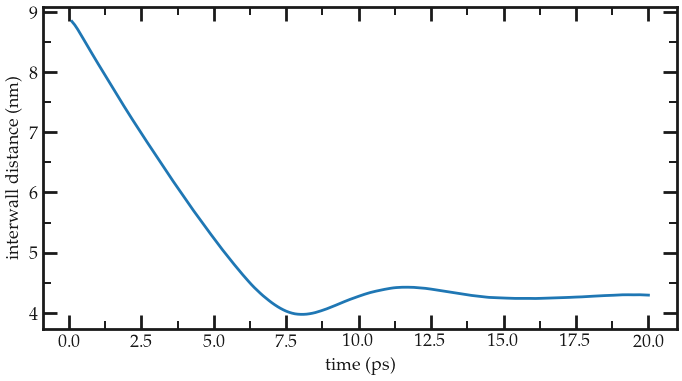
\includegraphics[width=\linewidth]{tutorials/level2/nanosheared-electrolyte/equilibration-light.png}
\end{figure}

Note that for actual reseach, it is recommended to run this equilibration step for longer times
to make sure that proper equilibration was reached. Here, since the slowest
process is the ionic diffusion, the equilibration 
should be longer than the typical diffusion time of the ions over the 
size of the pore (~3 nm), i.e. of the order of the nanosecond.

\section{Imposed shearing}

\noindent From the equilibrated configuration, let us impose the
motion of the two walls in order to shear the electrolyte.
In a new folder called \textit{Shearing/},
create a new input that starts like the previous ones:

\begin{lcverbatim}
# Initialisation
boundary p p p
units real
atom_style full
bond_style harmonic
angle_style harmonic
pair_style lj/cut/tip4p/long 1 2 1 1 0.1546 12.0
kspace_style pppm/tip4p 1.0e-4
# System definition
read_data ../Equilibration/system.data
change_box all z final -40 40
# Simulation settings
include ../PARM.lammps
# Groups
group gH2O type 1 2
group gNa type 3
group gCl type 4
group gliquid type 1 2 3 4
group gwall type 5
region rtop block INF INF INF INF 0 INF
region rbot block INF INF INF INF INF 0
group gtop region rtop
group gbot region rbot
group gwalltop intersect gwall gtop
group gwallbot intersect gwall gbot
# Dynamics
fix mynve all nve
compute tliq gliquid temp/partial 0 1 1
fix myber1 gliquid temp/berendsen 300 300 100
fix_modify myber1 temp tliq
compute twall gwall temp/partial 0 1 1
fix myber2 gwall temp/berendsen 300 300 100
fix_modify myber2 temp twall
fix myshk gH2O shake 1.0e-4 200 0 b 1 a 1
fix myrct all recenter NULL NULL INIT
\end{lcverbatim}

\noindent The main difference with the previous \textit{equilibration} step, so far, is
the use of temperature \textit{compute} with \textit{temp/partial 0 1 1} options.
This is meant to exclude the \textit{x} coordinate from the thermalisation, which is 
important since a large velocity will be imposed along \textit{x}. Another difference is the
\textit{change$\_$box} command used to reduce the size of the box along \textit{z} (otherwise there 
is too much unecessary vacuum).
Then, let us impose the motion of the two walls:

\begin{lcverbatim}
fix mysf1 gwalltop setforce 0 NULL NULL
fix mysf2 gwallbot setforce 0 NULL NULL
velocity gwallbot set -20e-5 NULL NULL
velocity gwalltop set 20e-5 NULL NULL
\end{lcverbatim}

\noindent The \textit{setforce} commands cancel the forces on a group of atoms at
every timestep, so the atoms of the group do not
experience any force from the rest of the system. In absence of force
acting on those atoms, they will conserve their initial velocity.
The \textit{velocity} commands act only once and impose
the velocity of the atoms of the groups \textit{gwallbot} and \textit{gwalltop}, respectively.
Finally, let us dump the atom positions, extract the
velocity profile using the ave/chunk command, extract the
force applied on the walls, and then run for 20 ps (feel free to increase the duration 
for more accurate velocity profile):

\begin{lcverbatim}
# vizualisation
dump mydmp all atom 5000 dump.lammpstrj
thermo 500
thermo_modify temp tliq
compute cc1 gliquid chunk/atom bin/1d z 0.0 1.0
fix myac1 gliquid ave/chunk 10 1500 20000 cc1 vx file vel.profile.dat
compute cc2 gwall chunk/atom bin/1d z 0.0 1.0
fix myac2 gwall ave/chunk 10 1500 20000 cc2 vx file vel.solid.dat
fix myat1 all ave/time 10 100 1000 f_mysf1[1] f_mysf2[1] file forces.dat
timestep 1.0
run 20000
write_data system.data
\end{lcverbatim}

\noindent Note that a duration of 20 ps is too short to measure meaningfull quantities.
If you computer allows it, use 200 ps instead.
The averaged velocity profile (with a 200 ps run) is the following:

\begin{figure}
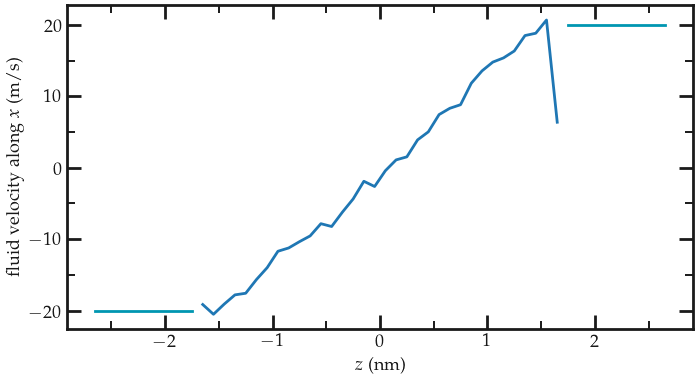
\includegraphics[width=\linewidth]{tutorials/level2/nanosheared-electrolyte/shearing-light.png}
\end{figure}

From the force applied by the fluid on the solid, one can
extract the stress within the fluid, which allows one to
measure its viscosity $\dot{\eta}$ 
according to \href{https://pure.tudelft.nl/ws/portalfiles/portal/89280267/PhysRevFluids.6.034303.pdf}{gravelle2021}:
$\eta = \tau / \dot{\gamma}$ where $\tau$
is the stress applied by the fluid on the shearing wall, and
$\dot{\gamma}$ the shear rate (which is imposed
here). Here the shear rate is approximatively 6.25e9
s-1, and using a surface area of 1e-17 m2, I
get a viscosity for the fluid equal to 2.25 mPa.s
The viscosity calculated at such high shear rate may
differ from the bulk value. In general, it is recommanded to use a lower
value for the shear rate. Note that for lower shear rate, the ratio noise-to-signal
is larger, and longer simulations must be performed.
Also note that the viscosity of a fluid next to a solid surface is
typically larger than in bulk due to interaction with the
walls. Therefore one expect the present simulation to return 
a viscosity that is slightly larger than what would be measured with 
the fluid alone.

\section{Going further with exercises}

\noindent \subsection{Density profiles}

Perform an equilibrium simulation, and extract both density
profiles and diffusion coefficients in all 3 directions of
space.
Hint: in general, data extraction can ne done either (1)
using the internal LAMMPS commands (e.g. variable/compute
+ fix ave/time), or (2) using a post-processing analysis
tool (e.g. Python).

\subsection{Poiseuille flow}

\noindent Instead of inducing shearing using the walls, induce a flow
of the liquid in the direction tangential to the walls, and
extract the the velocity profile.
Advice: the forcing must be chosen with care. If too
large, the system will be strongly out-of-equilibrium. If
too small, no net velocity will be measured because of
the thermal noise.
Question: Is the velocity profile you obtain consistent with
Poiseuille's predictions?

